\documentclass[11pt]{beamer}\usepackage[]{graphicx}\usepackage[]{color}
%% maxwidth is the original width if it is less than linewidth
%% otherwise use linewidth (to make sure the graphics do not exceed the margin)
\makeatletter
\def\maxwidth{ %
  \ifdim\Gin@nat@width>\linewidth
    \linewidth
  \else
    \Gin@nat@width
  \fi
}
\makeatother

\definecolor{fgcolor}{rgb}{0.345, 0.345, 0.345}
\newcommand{\hlnum}[1]{\textcolor[rgb]{0.686,0.059,0.569}{#1}}%
\newcommand{\hlstr}[1]{\textcolor[rgb]{0.192,0.494,0.8}{#1}}%
\newcommand{\hlcom}[1]{\textcolor[rgb]{0.678,0.584,0.686}{\textit{#1}}}%
\newcommand{\hlopt}[1]{\textcolor[rgb]{0,0,0}{#1}}%
\newcommand{\hlstd}[1]{\textcolor[rgb]{0.345,0.345,0.345}{#1}}%
\newcommand{\hlkwa}[1]{\textcolor[rgb]{0.161,0.373,0.58}{\textbf{#1}}}%
\newcommand{\hlkwb}[1]{\textcolor[rgb]{0.69,0.353,0.396}{#1}}%
\newcommand{\hlkwc}[1]{\textcolor[rgb]{0.333,0.667,0.333}{#1}}%
\newcommand{\hlkwd}[1]{\textcolor[rgb]{0.737,0.353,0.396}{\textbf{#1}}}%

\usepackage{framed}
\makeatletter
\newenvironment{kframe}{%
 \def\at@end@of@kframe{}%
 \ifinner\ifhmode%
  \def\at@end@of@kframe{\end{minipage}}%
  \begin{minipage}{\columnwidth}%
 \fi\fi%
 \def\FrameCommand##1{\hskip\@totalleftmargin \hskip-\fboxsep
 \colorbox{shadecolor}{##1}\hskip-\fboxsep
     % There is no \\@totalrightmargin, so:
     \hskip-\linewidth \hskip-\@totalleftmargin \hskip\columnwidth}%
 \MakeFramed {\advance\hsize-\width
   \@totalleftmargin\z@ \linewidth\hsize
   \@setminipage}}%
 {\par\unskip\endMakeFramed%
 \at@end@of@kframe}
\makeatother

\definecolor{shadecolor}{rgb}{.97, .97, .97}
\definecolor{messagecolor}{rgb}{0, 0, 0}
\definecolor{warningcolor}{rgb}{1, 0, 1}
\definecolor{errorcolor}{rgb}{1, 0, 0}
\newenvironment{knitrout}{}{} % an empty environment to be redefined in TeX

\usepackage{alltt}
\usetheme{Warsaw}
\usepackage[utf8]{inputenc}
\usepackage{amsmath}
\usepackage{amsfonts}
\usepackage{amssymb}
\usepackage{array}
\usepackage{graphicx}
\author{John Muschelli}
\usepackage{hyperref}
\setbeamertemplate{navigation symbols}{}%remove navigation symbols

\title{Image Processing with ANTsR}
%\setbeamercovered{transparent} 
%\setbeamertemplate{navigation symbols}{} 
%\logo{} 
\institute{Johns Hopkins Bloomberg School of Public Health} 
%\date{} 
%\subject{} 
\setlength{\topsep}{0pt}
\setlength{\parskip}{0pt}
\setlength{\partopsep}{1pt}
\setbeamertemplate{footline}[frame number]

\usepackage[
  natbib = true,
    backend=bibtex,
]{biblatex}
\bibliography{ANTsR}
\AtEveryBibitem{
\clearfield{note}
% \clearlist{address}
% \clearfield{eprint}
% \clearfield{isbn}
% \clearfield{issn}
% \clearlist{location}
% \clearfield{month}
% \clearfield{series}
} % clears language


\newcommand {\framedgraphic}[2] {
    \begin{frame}{#1}
        \begin{center}
            \includegraphics[width=\textwidth,height=0.8\textheight,keepaspectratio]{#2}
        \end{center}
    \end{frame}
}
\IfFileExists{upquote.sty}{\usepackage{upquote}}{}
\begin{document}

\begin{frame}
\titlepage
\end{frame}

%\begin{frame}
%\tableofcontents
%\end{frame}




\begin{frame}[fragile]{ANTS and ANTsR}

\begin{itemize}
\item Advanced normalization tools (ANTS) \citep{avants2011reproducible} is state-of-the art software that can perform many neuroimaging-related functions.  
	\begin{itemize}
	\item Collection of routines in C, C++, and some R
	\end{itemize}
\item ANTsR: port of ANTS into R using Rcpp
\item The two functions we focus on are: 
\begin{enumerate}
\item Image inhomogeneity correction (N3 \citep{sled1998nonparametric} and N4 \citep{tustison2010n4itk})
\item Image registration
\end{enumerate} 
\end{itemize}

\end{frame}


\begin{frame}[fragile]{Installing ANTsR}
ANTsR is currently (as of March 23, 2015) hosted on GitHub.  

We will install ANTsR using the \verb|devtools| package.  

Overall, any updates to the install process will be located at \href{https://github.com/stnava/ANTsR}{https://github.com/stnava/ANTsR}.

%This build requires \href{http://www.cmake.org/}{CMake}.

\begin{knitrout}
\definecolor{shadecolor}{rgb}{0.969, 0.969, 0.969}\color{fgcolor}\begin{kframe}
\begin{alltt}
\hlkwa{if} \hlstd{(}\hlopt{!}\hlkwd{require}\hlstd{(devtools))\{}
        \hlkwd{install.packages}\hlstd{(}\hlstr{'devtools'}\hlstd{)}
\hlstd{\}}
\hlstd{devtools}\hlopt{::}\hlkwd{install_github}\hlstd{(}\hlstr{"stnava/cmaker"}\hlstd{)}
\hlstd{devtools}\hlopt{::}\hlkwd{install_github}\hlstd{(}\hlstr{"stnava/ITKR"}\hlstd{)}
\hlstd{devtools}\hlopt{::}\hlkwd{install_github}\hlstd{(}\hlstr{"stnava/ANTsR"}\hlstd{)}
\end{alltt}
\end{kframe}
\end{knitrout}
\end{frame}

\begin{frame}[fragile]{Reading in Images using ANTsR}
Reading in images using ANTsR requires 2 changes compared to \verb|readNIfTI| from \verb|oro.nifti|:
\begin{enumerate}
\item The extension of the filename (e.g. \verb|.nii.gz|) must be specified
\item The dimension of the image (usually 3) must be supplied (could be 2, 3, or 4)
\end{enumerate}

\begin{knitrout}
\definecolor{shadecolor}{rgb}{0.969, 0.969, 0.969}\color{fgcolor}\begin{kframe}
\begin{alltt}
\hlkwd{library}\hlstd{(ANTsR)}
\hlstd{aimg} \hlkwb{=} \hlkwd{antsImageRead}\hlstd{(}\hlstr{"Output_3D_File.nii.gz"}\hlstd{,}
        \hlkwc{dimension} \hlstd{=} \hlnum{3}\hlstd{)}
\end{alltt}
\end{kframe}
\end{knitrout}
\end{frame}


\begin{frame}[fragile]{ANTsR images}

The \verb|aimg| object is an object of \verb|antsImage|, which consists of:
\begin{itemize}
\item pixeltype - how is the image stored (integers versus fractional numbers (floats))
\item dimension - how many dimensions does the image have
\item pointer - where the data is stored
\end{itemize}

\begin{knitrout}
\definecolor{shadecolor}{rgb}{0.969, 0.969, 0.969}\color{fgcolor}\begin{kframe}
\begin{alltt}
\hlkwd{class}\hlstd{(aimg)}
\end{alltt}
\begin{verbatim}
[1] "antsImage"
attr(,"package")
[1] "ANTsR"
\end{verbatim}
\begin{alltt}
\hlstd{aimg}
\end{alltt}
\begin{verbatim}
antsImage
  Pixel Type   : float 
  Pixel Size   : 1 
  Dimensions   : 512x512x22 
  Voxel Spacing: 0.46875x0.46875x5 
  Origin       : 0 0 0 
  Direction    : 1 0 0 0 -1 0 0 0 1 
\end{verbatim}
\begin{alltt}
\hlkwd{slotNames}\hlstd{(aimg)}
\end{alltt}
\begin{verbatim}
[1] "pixeltype"  "dimension"  "components" "pointer"   
\end{verbatim}
\end{kframe}
\end{knitrout}
\end{frame}


\begin{frame}[fragile]{ANTsR images: statistics}

We can still do statistics from an \verb|antsImage|:
\begin{knitrout}
\definecolor{shadecolor}{rgb}{0.969, 0.969, 0.969}\color{fgcolor}\begin{kframe}
\begin{alltt}
\hlkwd{mean}\hlstd{(aimg)}
\end{alltt}
\begin{verbatim}
[1] 102.4701
\end{verbatim}
\begin{alltt}
\hlkwd{mean}\hlstd{(aimg[aimg}\hlopt{!=}\hlnum{0}\hlstd{])}
\end{alltt}
\begin{verbatim}
[1] 179.4116
\end{verbatim}
\end{kframe}
\end{knitrout}
and get the image data from an \verb|antsImage| using \verb|as.array|:

\begin{knitrout}
\definecolor{shadecolor}{rgb}{0.969, 0.969, 0.969}\color{fgcolor}\begin{kframe}
\begin{alltt}
\hlkwd{class}\hlstd{(}\hlkwd{as.array}\hlstd{(aimg))}
\end{alltt}
\begin{verbatim}
[1] "array"
\end{verbatim}
\end{kframe}
\end{knitrout}

\end{frame}

\begin{frame}[fragile]{But we discussed nifti objects before!?}

Why discuss the \verb|antsImage| class?

\begin{enumerate}
\item The class can be very fast at performing operations
\item Some ANTsR functions return object of \verb|antsImage| class
\item Some ANTsR functions require an object of \verb|antsImage| class as input
\end{enumerate}

\end{frame}


\begin{frame}[fragile]{Partial Solution: Use extrantsr}

The \verb|extrantsr| (EXTRa ANTsR) package has helper functions to jump \verb|ANTsR| and the \verb|oro.nifti| classes:

Installing \verb|extrantsr|:
\begin{knitrout}
\definecolor{shadecolor}{rgb}{0.969, 0.969, 0.969}\color{fgcolor}\begin{kframe}
\begin{alltt}
\hlstd{devtools}\hlopt{::}\hlkwd{install_github}\hlstd{(}\hlstr{"muschellij2/extrantsr"}\hlstd{)}
\end{alltt}
\end{kframe}
\end{knitrout}
\begin{knitrout}
\definecolor{shadecolor}{rgb}{0.969, 0.969, 0.969}\color{fgcolor}\begin{kframe}
\begin{alltt}
\hlkwd{library}\hlstd{(extrantsr)}
\hlkwd{class}\hlstd{(nim} \hlkwb{<-} \hlkwd{ants2oro}\hlstd{(aimg))}
\end{alltt}
\begin{verbatim}
[1] "nifti"
attr(,"package")
[1] "oro.nifti"
\end{verbatim}
\end{kframe}
\end{knitrout}

\end{frame}


\begin{frame}[fragile]{Wrapper functions in extrantsr: Bias Field Correction}

\verb|extrantsr::bias_correct| wraps \verb|n3BiasFieldCorrection| \citep{sled1998nonparametric} and \verb|n4BiasFieldCorrection| \citep{tustison2010n4itk} from \verb|ANTsR| for bias field correction:

\begin{knitrout}
\definecolor{shadecolor}{rgb}{0.969, 0.969, 0.969}\color{fgcolor}\begin{kframe}
\begin{alltt}
\hlstd{n3img} \hlkwb{=} \hlkwd{bias_correct}\hlstd{(nim,} \hlkwc{correction} \hlstd{=} \hlstr{"N3"}\hlstd{,}
        \hlkwc{retimg}\hlstd{=}\hlnum{TRUE}\hlstd{)}
\hlstd{n4img} \hlkwb{=} \hlkwd{bias_correct}\hlstd{(nim,} \hlkwc{correction} \hlstd{=} \hlstr{"N4"}\hlstd{,}
        \hlkwc{retimg}\hlstd{=}\hlnum{TRUE}\hlstd{)}
\end{alltt}
\end{kframe}
\end{knitrout}
\end{frame}



\begin{frame}[fragile]{Wrapper functions in extrantsr: Bias Field Correction}

\begin{tabular}{cc}
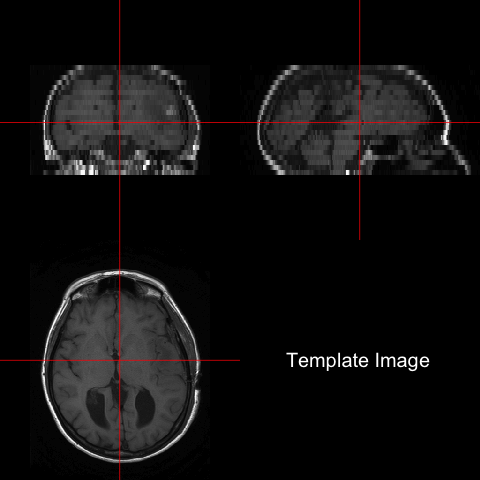
\includegraphics[width=0.5\linewidth]{Orig_Image.png} & 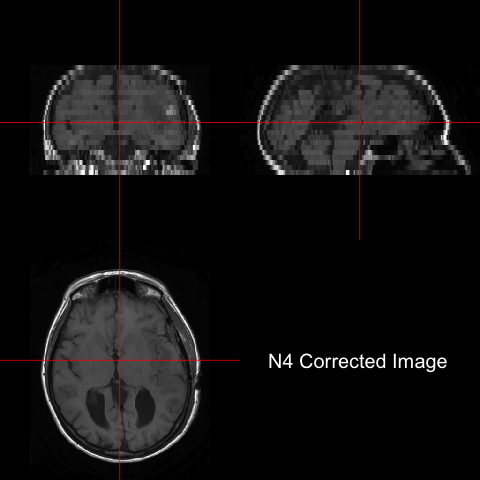
\includegraphics[width=0.5\linewidth]{N4_Image.png}
\end{tabular}

\end{frame}

\begin{frame}[fragile]{Wrapper functions in extrantsr: Image Registration}

\begin{itemize}
\item \verb|ANTsR| worker function: \verb|antsRegistration|
\item \verb|extrantsr| worker function: \verb|ants_regwrite|
\end{itemize}
\verb|ants_regwrite| takes in a filename and a template filename, other files (in the same space as filename) to transform to template:
\begin{knitrout}
\definecolor{shadecolor}{rgb}{0.969, 0.969, 0.969}\color{fgcolor}\begin{kframe}
\begin{alltt}
\hlstd{registered_n4} \hlkwb{=} \hlkwd{ants_regwrite}\hlstd{(}\hlkwc{filename}\hlstd{=n4img,}
        \hlkwc{template.file} \hlstd{=} \hlstr{"MNI152_T1_1mm.nii.gz"}\hlstd{,}
        \hlkwc{remove.warp} \hlstd{=} \hlnum{TRUE}\hlstd{,}
        \hlkwc{typeofTransform} \hlstd{=} \hlstr{"Rigid"}\hlstd{)}
\end{alltt}
\end{kframe}
\end{knitrout}
\end{frame}



\begin{frame}[fragile]{Wrapper functions in extrantsr: Image Registration}

\begin{tabular}{cc}
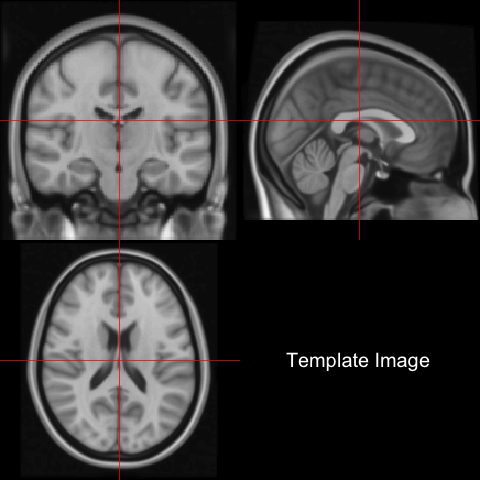
\includegraphics[width=0.5\linewidth]{Template.png} & 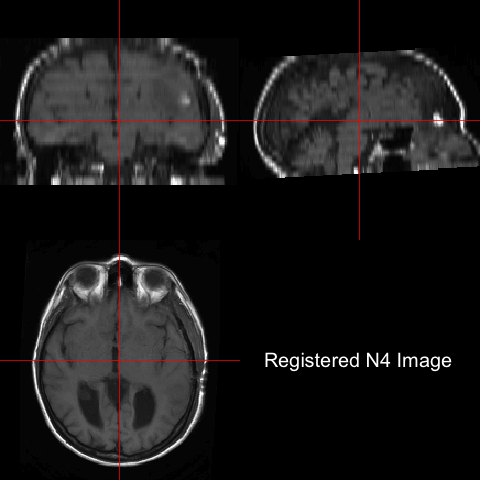
\includegraphics[width=0.5\linewidth]{Reg_Image.png}
\end{tabular}

\end{frame}

\begin{frame}[t,allowframebreaks]
  \frametitle{References}
  \printbibliography
 \end{frame}
 
\end{document}
